\item \textbf{{[}RVHS/PRELIM/9597/2018/P1/Q4{]} }

\textbf{Reversi }

In this task you will implement part of the board game called Reversi. 

\subsection*{Task 4.1 }

Implement the function \texttt{initiate\_board} which takes in an
integer \texttt{size} and returns a 2-dimension list that contains
\texttt{size} $\times$ \texttt{size} \textquotedbl{} \textquotedbl .

For example, 

\noindent %
\noindent\begin{minipage}[t]{1\columnwidth}%
\texttt{>\textcompwordmark >\textcompwordmark > initiate\_board(2)}

\texttt{{[}{[}' ', ' '{]}, {[}' ', ' '{]}{]} }

\texttt{>\textcompwordmark >\textcompwordmark > initiate\_board(10) }

\texttt{{[}{[}' ', ' ', ' ', ' ', ' ', ' ', ' ', ' ', ' ', ' '{]},}

\texttt{~{[}' ', ' ', ' ', ' ', ' ', ' ', ' ', ' ', ' ', ' '{]}, }

\texttt{~{[}' ', ' ', ' ', ' ', ' ', ' ', ' ', ' ', ' ', ' '{]}, }

\texttt{~{[}' ', ' ', ' ', ' ', ' ', ' ', ' ', ' ', ' ', ' '{]}, }

\texttt{~{[}' ', ' ', ' ', ' ', ' ', ' ', ' ', ' ', ' ', ' '{]}, }

\texttt{~{[}' ', ' ', ' ', ' ', ' ', ' ', ' ', ' ', ' ', ' '{]}, }

\texttt{~{[}' ', ' ', ' ', ' ', ' ', ' ', ' ', ' ', ' ', ' '{]},}

\texttt{~{[}' ', ' ', ' ', ' ', ' ', ' ', ' ', ' ', ' ', ' '{]},}

\texttt{~{[}' ', ' ', ' ', ' ', ' ', ' ', ' ', ' ', ' ', ' '{]},}

\texttt{~{[}' ', ' ', ' ', ' ', ' ', ' ', ' ', ' ', ' ', ' '{]}{]}}%
\end{minipage}

\subsection*{Evidence 18}

Program code of \texttt{initiate\_board}. \hfill{}{[}1{]}

\subsection*{Task 4.2}

Implement the function display\_board which takes in a 2-dimension
list board and output the playboard following the format below. For
example, 

\noindent %
\noindent\begin{minipage}[t]{1\columnwidth}%
\texttt{>\textcompwordmark >\textcompwordmark > b1 = {[}{[}'X',
' ', 'O'{]}, {[}' ', 'X', ' '{]}, {[}'O', 'X', 'O'{]}{]}}

\texttt{>\textcompwordmark >\textcompwordmark > display\_board(b1) }

\texttt{-{}-0-1-2- }

\texttt{0|X| |O| }

\texttt{1| |X| | }

\texttt{2|O|X|O| }

\texttt{>\textcompwordmark >\textcompwordmark > b2 = {[}{[}\textquotedbl{}
\textquotedbl ,\textquotedbl{} \textquotedbl ,\textquotedbl{} \textquotedbl ,\textquotedbl{}
\textquotedbl ,\textquotedbl{} \textquotedbl ,\textquotedbl{} \textquotedbl ,\textquotedbl{}
\textquotedbl ,\textquotedbl{} \textquotedbl{]}, }

\texttt{~~~~~~~~~~{[}\textquotedbl{} \textquotedbl ,\textquotedbl{}
\textquotedbl ,\textquotedbl{} \textquotedbl ,\textquotedbl{} \textquotedbl ,\textquotedbl{}
\textquotedbl ,\textquotedbl{} \textquotedbl ,\textquotedbl{} \textquotedbl ,\textquotedbl{}
\textquotedbl{]}, }

\texttt{~~~~~~~~~~{[}\textquotedbl{} \textquotedbl ,\textquotedbl{}
\textquotedbl ,\textquotedbl{} \textquotedbl ,\textquotedbl{} \textquotedbl ,\textquotedbl{}
\textquotedbl ,\textquotedbl{} \textquotedbl ,\textquotedbl{} \textquotedbl ,\textquotedbl{}
\textquotedbl{]}, }

\texttt{~~~~~~~~~~{[}\textquotedbl{} \textquotedbl ,\textquotedbl{}
\textquotedbl ,\textquotedbl{} \textquotedbl ,\textquotedbl X\textquotedbl ,\textquotedbl O\textquotedbl ,\textquotedbl{}
\textquotedbl ,\textquotedbl{} \textquotedbl ,\textquotedbl{} \textquotedbl{]}, }

\texttt{~~~~~~~~~~{[}\textquotedbl{} \textquotedbl ,\textquotedbl{}
\textquotedbl ,\textquotedbl{} \textquotedbl ,\textquotedbl O\textquotedbl ,\textquotedbl X\textquotedbl ,\textquotedbl{}
\textquotedbl ,\textquotedbl{} \textquotedbl ,\textquotedbl{} \textquotedbl{]}, }

\texttt{~~~~~~~~~~{[}\textquotedbl{} \textquotedbl ,\textquotedbl{}
\textquotedbl ,\textquotedbl{} \textquotedbl ,\textquotedbl{} \textquotedbl ,\textquotedbl{}
\textquotedbl ,\textquotedbl{} \textquotedbl ,\textquotedbl{} \textquotedbl ,\textquotedbl{}
\textquotedbl{]}, }

\texttt{~~~~~~~~~~{[}\textquotedbl{} \textquotedbl ,\textquotedbl{}
\textquotedbl ,\textquotedbl{} \textquotedbl ,\textquotedbl{} \textquotedbl ,\textquotedbl{}
\textquotedbl ,\textquotedbl{} \textquotedbl ,\textquotedbl{} \textquotedbl ,\textquotedbl{}
\textquotedbl{]}, }

\texttt{~~~~~~~~~~{[}\textquotedbl{} \textquotedbl ,\textquotedbl{}
\textquotedbl ,\textquotedbl{} \textquotedbl ,\textquotedbl{} \textquotedbl ,\textquotedbl{}
\textquotedbl ,\textquotedbl{} \textquotedbl ,\textquotedbl{} \textquotedbl ,\textquotedbl{}
\textquotedbl{]}{]} }

\texttt{>\textcompwordmark >\textcompwordmark > display\_board(b2) }

\texttt{-{}-0-1-2-3-4-5-6-7- }

\texttt{0| | | | | | | | | }

\texttt{1| | | | | | | | | }

\texttt{2| | | | | | | | | }

\texttt{3| | | |X|O| | | | }

\texttt{4| | | |O|X| | | | }

\texttt{5| | | | | | | | | }

\texttt{6| | | | | | | | | }

\texttt{7| | | | | | | | |}

\texttt{-{}-{}-{}-{}-{}-{}-{}-{}-{}-{}-{}-{}-{}-{}-{}-{}-{}- }%
\end{minipage}

\subsection*{Evidence 19 }

Program code of \texttt{display\_board}.\hfill{} {[}4{]}

\subsection*{Task 4.3 }

Implement the function \texttt{reverse} which simulates a valid move
in the game Reversi.

It takes in 4 parameters as shown below. 
\begin{itemize}
\item \texttt{board} -- a 2-Dimension list that represents the current
state of the play board.
\item \texttt{row} -- an integer that represents the row number at which
the disc is placed. 
\item \texttt{col} -- an integer that represents the column number at which
the disc is placed. 
\item \texttt{disc} -- a string that takes either the value of \textquotedbl X\textquotedbl{}
or \textquotedbl O\textquotedbl{} which represents black and white
of the disc. 
\end{itemize}
The function returns \texttt{True} if it is a valid move and then
updates \texttt{board} accordingly, otherwise, returns \texttt{False}
without updating \texttt{board}. 

A valid move refers to, for example, placing a \textquotedblleft \texttt{X}\textquotedblright{}
disc at a position that there exists at least one straight (horizontal,
vertical, or diagonal) occupied line between the new piece and another
\textquotedblleft \texttt{X}\textquotedblright{} piece, with one or
more contiguous \textquotedblleft \texttt{O}\textquotedblright{} pieces
between them, and vice versa. 

\textbf{Examples }
\begin{center}
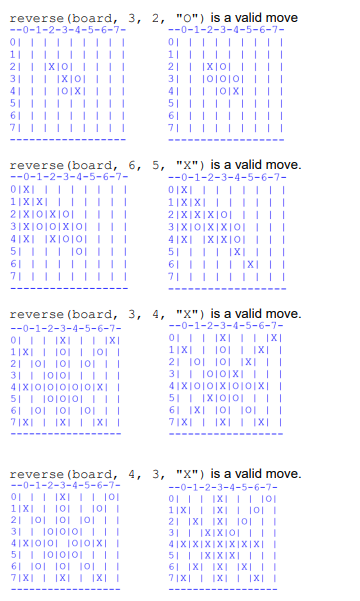
\includegraphics[width=0.5\paperwidth]{C:/Users/Admin/Desktop/Github/question_bank/LyX/static/img/9597-RVHS-2018-P1-Q4-1}
\par\end{center}

\subsection*{Evidence 20}

Program code of the iterative version of function \texttt{reverse}.
\hfill{}{[}5{]}

Program code of the recursive version of function \texttt{reverse}.
\hfill{}{[}5{]}